\documentclass[14pt, a4paper, titlepage, fleqn]{extarticle}

\usepackage{style/style}
\usepackage{style/titlepage}

\everymath{\displaystyle}

\title{Контрольная работа по решению уравнений и систем уравнений}
\author{Держапольский Юрий Витальевич \\ Группа Б9121-01.03.02сп}
\date{}

\begin{document}

    \maketitle

    \section*{Задание 1}
        Выписать формулу метода Ньютона для поиска корня нелинейного уравнения. Начальное приближение к корню определить графически. Оценить априорно число итераций, необходимое для достижения точности \( \varepsilon = 0.00001 \): \\
        \( e^x - 2x - 2 = 0 \)
    \section*{Решение}
        Формула метода Ньютона:
        \( \varphi(x) = x - \frac{f(x)}{f'(x)} = x - \frac{e^{x} - 2x - 2}{e^{x} - 2} \)
        
        \begin{figure}[H]
            \centering
            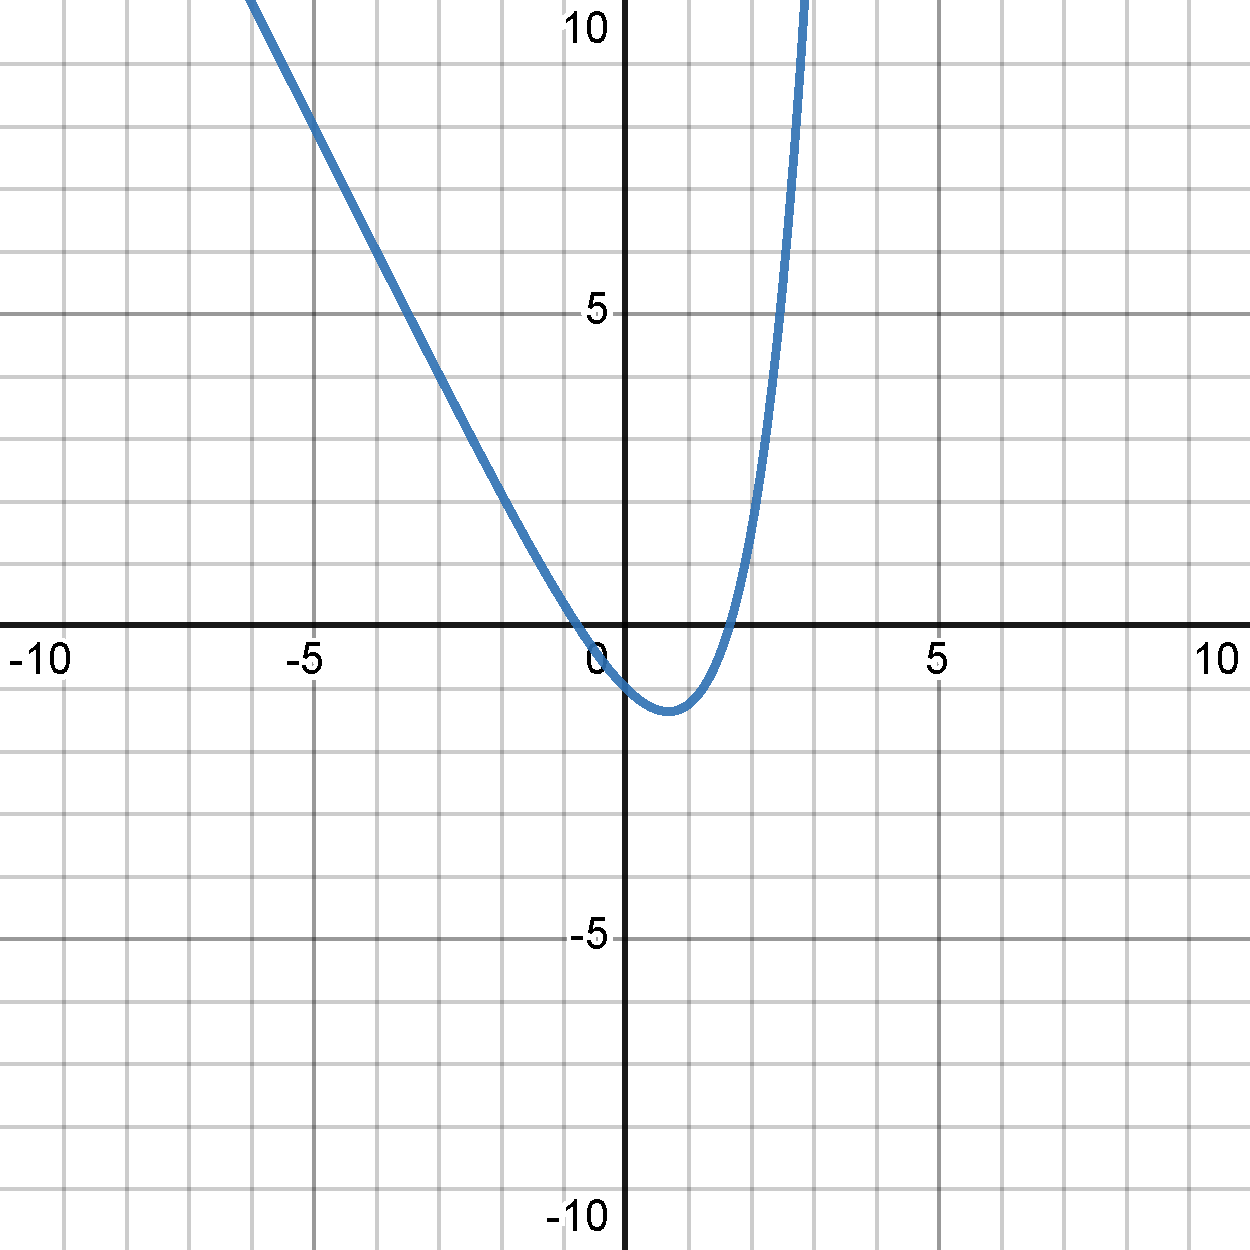
\includegraphics[width=7cm]{z1.pdf}
            \caption{График функции}
        \end{figure}

        Возьмём для поиска положительный корень \( x^* \approx 1.678437\dots \) и начальное приближение \( x_0 = 2 \). Оценим число итераций.

        Используем оценку \( | x_n - x^* | \leq \left| \frac{\varphi''(x^*)}{2} (x_{n-1} - x^*)^2 \right| \). Последовательно применяя оценку, получим: \( | x_n - x^* | \leq \left| \left(\frac{\varphi''(x^*)}{2} \right)^{2^n -1} (x_{0} - x^*)^{2^n} \right| \leq 10^{-5} \). Откуда можно найти \( n \geq 3.1 \). Значит что 4-мя итерациями мы найдём корень с точностью до \( \varepsilon = 10^{-5} \).

\end{document}